\section{Background: Goal-oriented Requirements Language and Argument Schemes}
\label{sect:background}

In this section, we first introduce and motivate the Goal-oriented Requirements Language (GRL), which is the goal modeling language used to connect to the argumentation framework. Next, we introduce and motivate \emph{the Argument Scheme for Practical Reasoning} (PRAS), which is a particular argument scheme that is used to form arguments and counter-arguments about situations involving goals.

\subsection{Goal-oriented Requirements Language (GRL)}
\label{sect:background:grl}
GRL is a visual modeling language for specifying intentions, business goals, and non-functional requirements (NFRs) of multiple stakeholders \cite{Amyot:2010:EGM:1841349.1841356}. It can be used to specify alternatives that have to be considered, decisions that have been made, and rationales for making decisions. A GRL model is a connected graph of intentional elements that optionally are part of actors. Figure~\ref{fig:trafficsim} illustrates a GRL diagram. An actor (
\includegraphics[scale=1]{img/actor}) represents a stakeholder of a system (\textbf{User}, Figure~\ref{fig:trafficsim}), or the system itself (\textbf{Simulation}, Figure~\ref{fig:trafficsim}). Actors are holders of intentions; they are the active entities in the system or its environment who want goals to be achieved, tasks to be performed, resources to be available, and softgoals to be satisfied. Softgoals (
\includegraphics[scale=1]{img/softgoal}) differentiate themselves from goals (
\includegraphics[scale=1]{img/goal}) in that there is no clear, objective measure of satisfaction for a softgoal whereas a goal is quantifiable, often in a binary way. Softgoals (e.g. \textbf{Realistic simulation)} are often more related to NFRs, whereas goals (such as \textbf{Generate cars}) are more related to functional requirements. Tasks (
\includegraphics[scale=1]{img/task}) represent solutions to (or operationalizations of) goals and softgoals. In Figure~\ref{fig:trafficsim}, some of the tasks are \textbf{Create new cars} and \textbf{Keep same cars}. In order to be achieved or completed, softgoals, goals, and tasks may require resources (
\includegraphics[scale=1]{img/resource}) to be available (e.g. \textbf{******})

\begin{figure*}[ht]
\centering
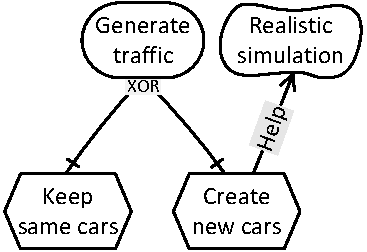
\includegraphics[scale=0.35]{img/Example}
\caption{GRL Model for the traffic simulator}
\label{fig:trafficsim}
\end{figure*}

Different links connect the elements in a GRL model. AND, IOR, and XOR decomposition links (
\includegraphics[scale=1]{img/decomposition}) allow an element to be decomposed into sub-elements. In Figure~\ref{fig:trafficsim}, the goal \textbf{Generate cars} is XOR-decomposed to the tasks \textbf{Create new cars} and \textbf{Keep same cars}. Contribution links (
\includegraphics[scale=1]{img/contribution}) indicate desired impacts of one element on another element. A contribution link has a qualitative contribution type or a quantitative contribution. Task \textbf{Create new cars} has a \textbf{help} qualitative contribution to the softgoal \textbf{Realistic simulation}. Dependency links (
\includegraphics[scale=1]{img/dependency}) model relationships between actors. For example, actor \textbf{Simulation} depends on the actor \textbf{User} to perform the task \textbf{Adjust car spawning rate} to fulfil its task \textbf{Create new cars}.

GRL is based on $i*$~\cite{Yu:1997:TMR:827255.827807} and the NFR Framework~\cite{chung2012non}, but it is not as restrictive as $i*$. Intentional elements and links can be more freely combined, the notion of agents is replaced with the more general notion of actors, i.e., stakeholders, and a task does not necessarily have to be an activity performed by an actor, but may also describe properties of a solution. GRL has a well-defined syntax and semantics, which are necessary if we want to incorporate it into a formal framework (requirements 1 and 2 as described in the introduction). Furthermore,GRL provides support for providing a scalable and consistent representation of multiple views/diagrams of the same goal model (see~\cite[Ch.2]{Ghanavati2013} for an more details). For example, traceability links are provided between between concepts and instances of goal modeling and behavioral design models \cite{}. Multiple views and traceability are a good fit with our current research: we aim to add traceability links between intentional elements and their underlying arguments. \todo{Sepideh}{Sepideh}{I need to improve: GRL has has the capability to be extended via profile, metadata and rules, and due to this capability, it has been extended to many domain. This feature also helps us to apply our argumentation to other domain such as compliance or enterprise architecture. }

\subsubsection{Traffic simulator example}
\label{sect:background:casestudy}

In this paper, we use the classic example of an online meeting scheduler that has been used in the literature~\cite{}, ~\cite{}, ~\cite{} several times. The meeting scheduler has been modeled with Tropos~\cite{} and $i*$. We remodel this example with GRL in jUCMNav for the purpose of our framework. 

The meeting scheduler system has three actors, \textbf{Meeting Initiator}, \textbf{Meeting Scheduler} and \textbf{Meeting Participant}. The \textbf{Meeting Scheduler} has a goal that for every meeting request, it has to try to find the best time and location in a way that most of the intended participants (i.e. \textbf{Meeting Participant}) can attend the meeting. The \textbf{Meeting Initiator} organizes the meetings by asking the participants to give their availability for a range of dates and time as well as the dates that they are not available. Based on these information, the \textbf{Meeting Scheduler} needs to pick a date/time and a location from the available dates/times given by the participants in a way that the most number of participants can attend. Participants should then accept or reject the event. 

The GRL model in Figure~\ref{fig:trafficsim} shows the softgoals, goals, tasks and the relationship between the different intentional elements in the model. However, the rationales and arguments behind certain intentional elements have not been discussed or illustrated in the GRL model. Some of the questions that might be interesting to know about are the following:

\todo{Sepideh}{Marc}{I think you can add some more or remove/modify some of these based on your needs in the future sections}
\begin{itemize}
	\item Why are only the two softgoals \textbf{Quick} and \textbf{Low effort} selected for the task \textbf{Organize Meeting}? Why is, for example, a goal \textbf{Selecting the most convenient time} not included in the analysis for the actor \textbf{Meeting Initiator}?
	\item What does \textbf{Quality of Proposed Date} mean?
	\item How can one decide if the quality is low or high? Who is in charge? \todo{Floris}{Sepideh}{do you mean the \textbf{Quality of Proposed Date}? Or quality of the GRL diagram?}
	\item Does the meeting initiator use an email to inform the meeting participants to enter their availabilities? 
	\item Does the meeting scheduler uses an online calendar to obtain the available dates or an online website?
	\item How much time do the participants have to enter their availabilities? Is that important? Do they get a reminder from either the initiator or the scheduler? Is the reminder sent via an email? 
	\item What does \textbf{Richer Medium} mean? 
\end{itemize}

\todo[resolved]{Sepideh}{all}{We need to further improve this part}
\todo{Marc}{all}{Improved this part, what do you think?}
These are the type of the questions that we cannot answer just by looking at the GRL models. The model in figure~\ref{fig:trafficsim} does not contain information about discussions that let up to the resulting elements of the model, such as by various clarification steps for the naming, or alternatives that have been considered for the relationships. In order to address this, we use Argument Schemes for Goal Modeling (GMAS). GMAS can help us decide what intentional elements should remain in GRL and what new ones to be added or deleted, provide rationale behind the design decisions and the relationships between the links. 

\subsection{Argument Scheme for Practical Reasoning (PRAS)}
\label{sect:background:pras}

Reasoning about which goals to pursue and actions to take is often referred to as \emph{practical reasoning}, and has been studied extensively in philosophy (e.g. \cite{Raz1978-RAZPR,walton1990}) and Artificial Intelligence \cite{Bratman1987,atkinson2007}. One approach is to capture practical reasoning in terms of arguments schemes and critical questions~\cite{walton1990}. The idea is that an instantiation of such a scheme gives a presumptive argument in favor of, for example, taking an action. This argument can then be tested by posing critical questions about, for instance, whether the action is possible given the situation, and a negative answer to such a question leads to a counterargument to the original presumptive argument for the action. 

A formal approach to persuasive and deliberative reasoning about goals and actions has been presented by Atkinson et al.~\cite{atkinson2007}, who define the Practical Reasoning Argument Scheme (PRAS). PRAS follows the following basic argument structure. 
\begin{equation}
\label{eq:eq1}
  \begin{aligned}
 \qquad&\text{I have goal } G&\\
&\text{Doing action }A \text{ will realize goal }G&\\
&\text{Which will promote value }V&\\
&\text{\emph{Therefore} I should do action }A.&
  \end{aligned}
\end{equation}

So, for example, we can say that 
\begin{itemize}
\item[] \textbf{Find agreeable meeting date} is a goal,
\item[] \textbf{Find agreeable date by talking to initiator} will realize the goal \textbf{(Find) agreeable meeting date},
\item[] Which will promote the value \textbf{User friendliness}
\item[] \textit{Therefore} 
\item[] We should perform action \textbf{Find agreeable date by talking to initiator}
\end{itemize}

Practical reasoning is defeasible, in that conclusions which are at one point acceptable can later be rejected because of new information. Atkinson \emph{et al.}~\cite{atkinson2007} define a set of critical questions that point to typical ways in which a practical argument can be criticized by, for example, questioning the validity of the elements in the scheme or the connections between the elements. Some examples of critical questions are as follows.

\begin{enumerate}
\item Will the action bring about the desired goal?
%\item Does the goal promote the value stated?
\item Are there alternative ways of realizing the same goal?
\item Are there alternative ways of promoting the same value?
%\item Does doing the action have a side effect which demotes the value?
\item Does doing the action have a side effect which demotes some other value?
\item Does doing the action promote some other value?
%\item Does doing the action preclude some other action which would promote some other value?
\item Is the action possible?
\item Can the desired goal be realized?
\item Is the value indeed a legitimate value?
\end{enumerate}

These critical questions can point to new arguments that might counter the original argument. Take, for example, critical question 8. If new evidence comes up indicating that meeting schedulers do not care about user friendliness we have a counterargument to the above argument, `evidence shows that \textbf{user friendliness} is not a legitimate value'. Another way to counter an argument for an action is to suggest an alternative action that realizes the same goal (question 2) or an alternative goal that promotes the same value (question 3). For example, we can argue that \textbf{Find agreeable date using scheduler} also realizes the goal \textbf{Find agreeable meeting date}, which gives us a counterargument to the original argument -- to find a date by talking to the initiator -- that also follows PRAS. 

In argumentation, counterarguments are said to \emph{attack} the original arguments (and sometimes vice versa). In the work of Atkinson et al.~\cite{atkinson2007}, arguments and their attacks are captured as an \emph{argumentation framework} of arguments and attack relations as introduced by Dung~\cite{Dung1995}\footnote{Full definitions of Dung's~\cite{Dung1995} frameworks and semantics will be given in section \ref{sect:gmas}. In this section, we will briefly discuss the intuitions behind these semantics.}. Figure \ref{fig:pras:example1} shows an argumentation framework with three arguments from the above example: the argument for \textbf{Find agreeable date by talking to initiator} (A1), the argument for \textbf{Find agreeable date using scheduler} (A3), and the argument that \textbf{User friendliness} is not a legitimate value (A2). The two alternative PRAS instantiations are A1 and A3. These arguments mutually attack each other, as \textbf{Find agreeable date by talking to initiator}  and \textbf{Find agreeable date using scheduler} are considered to be mutually exclusive. Argument A2 attacks A1, as it questions the legitimacy of the value \textbf{User friendliness}. 

\begin{figure}[ht]
\centering
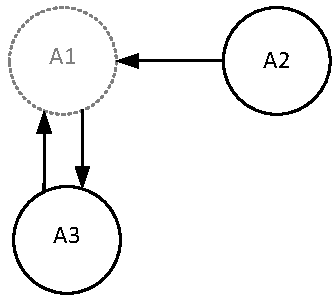
\includegraphics[scale=0.8]{img/Fig1}
\caption{Argumentation framework}
\label{fig:pras:example}
\end{figure}

Given an argumentation framework, the acceptability of arguments can be determined according to the appropriate argumentation semantics. The intuition is that an argument is acceptable if it is \emph{undefeated}, that is, any argument that attacks it, is itself defeated. In the argumentation framework in Figure~\ref{fig:pras:example}, argument A2 is undefeated because it has no attackers. This makes A1 defeated, because one of its attackers, A2, is undefeated. A3 is then also undefeated, since its only attacker, A1, is defeated by A2. Thus, the set of undefeated (justified) arguments given the argumentation framework in Figure~\ref{fig:pras:example} is $\{$A2, A3$\}$. 

In some cases, it is more difficult to determine whether or not an argument is defeated. Take, for example, the argumentation framework with just A1 and A3: they attack each other, they are alternatives and without any explicit preference, it is impossible to choose between the two. It is, however, possible to include explicit preferences between arguments when determining argument acceptability \cite{amgoud2002reasoning}. Take, for example, A1 and A3. If we say that we prefer the action \textbf{Find agreeable date by talking to initiator} (A1) over the action \textbf{Find agreeable date using scheduler} (A3), we remove the attack from A1 to A3 (Figure~\ref{fig:pras:example2}, left). This makes A1 the only undefeated argument, whereas A3 is now defeated. It is also possible to give explicit arguments for preferences \cite{modgil2009}. These arguments are then essentially attacks on attacks. For example, say we prefer A1 over A3 because `the \textbf{Meeting participant} does not like working with a scheduler' (A4). This can be rendered as a separate argument that attacks the attack from A3 to A1 (Figure~\ref{fig:pras:example2}, right), removing this attack and making $\{$A1, A4$\}$ the undefeated justified set of arguments.

\begin{figure}[ht]
\centering
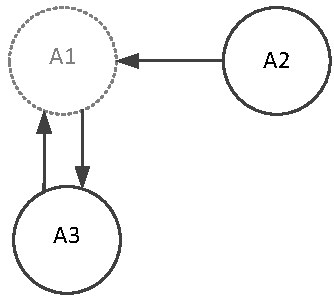
\includegraphics[scale=0.8]{img/Fig2}
\caption{Preferences between arguments}
\label{fig:pras:example2}
\end{figure}  

\subsubsection{Practical Argumentation and Goal Modeling}
\label{sect:background:pras:motivation}

Practical reasoning in the PRAS framework as described above provides a formally sound framework for defeasible reasoning about goals and actions that adheres to the acceptability semantics of Dung~\cite{Dung1995} and its various extensions \cite{amgoud2002reasoning,modgil2009}. The usefulness of PRAS for the analysis of practical reasoning situations has been shown in different areas such as e-democracy~\cite{cartwright2009IS}, law~\cite{atkinson2005legal}, planning \cite{medellin2013planning} and choosing between safety critical actions \cite{tolchinsky2012deliberation}. The question in this paper is how PRAS can be adopted for use in goal modeling, so that we can capture the discussions between stakeholders that build a goal model as formal argumentation, thus adding a new evaluation technique for goal models that allows us to assess the \emph{acceptability} of elements of a goal model (as opposed to the \emph{satisfiability} \todo{Marc}{Floris}{Which article do you want to cite here?}\cite{}).

\todo{Marc}{Floris}{From here on you seem to be discussing related work. This kind of distracts us from the main point of this article, and the section becomes quite long. Perhaps it is better to make the main arguments about why our approach is useful here, and move the discussion of our previous work and Jureta to related work?}

PRAS (actions, goals, values) and GRL (tasks, goals, softgoals) have some obvious similarities, and in previous work \cite{vanzee-etal:renext2015,vanZee-etal:er2016,vanZee-etal:comma2016} we presented arguments based on PRAS of the form ``G is a goal, Action A realizes G \emph{Therefore} perform action A'' (see Figure~\ref{fig:pras:example3}, left, where the arrow denotes an inference step). Such arguments, which can be constructed using the online OVA tool\footnote{\url{http://ova.arg-tech.org/}}, can be combined with further arguments providing, for example, expert opinions about the practical reasoning elements (Figure~\ref{fig:pras:example3}, left).

\begin{figure}[ht]
\centering
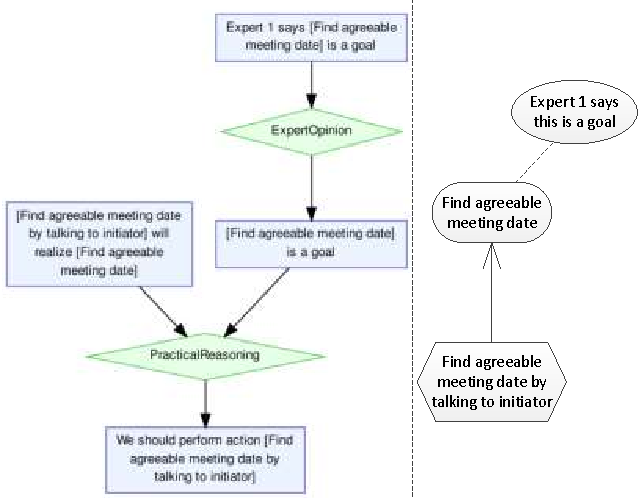
\includegraphics[width=\columnwidth]{img/Fig3}
\caption{Structured argument based on PRAS (left) and the corresponding GRL diagram (right)}
\label{fig:pras:example3}
\end{figure}  


Arguments built in OVA can automatically be translated to GRL diagrams using further online tooling\footnote{\url{https://github.com/RationalArchitecture/RationalGRL}} \cite{vanZee-etal:comma2016}. This translation takes the elements of the arguments and directly translates this to GRL elements. Tasks/actions, goals and softgoals/values can be directly translated from the arguments to the GRL diagrams, as can realization statements. Elements of arguments that have nothing to do with goal modelling (e.g. the expert opinion premise in Figure~\ref{fig:pras:example3}) can be included in the GRL diagram as \emph{beliefs}. Finally, attacks between arguments are captured as negative contribution links. Take, for example, \todo{example}. A very similar approach to argumentation and goal models had already been taken by Jureta et al.~\cite{Jureta:RE2008} who proposed a formal argumentation model that can be used to justify goal-modelling decisions. This argumentation model, while not explicitly based on a practical reasoning scheme, is essentially the same as our previous argumentation model based on PRAS: a formal model of structured arguments with goals as premises and tasks as conclusions, and a translation function of these arguments to goal diagrams. 

The core problem of the use of argumentation in the above-mentioned work \cite{Jureta:RE2008,vanzee-etal:renext2015,vanZee-etal:er2016}, is that it focuses mainly on structured arguments, which are then directly translated to goal models as in Figure~\ref{fig:pras:example3}. The question is what the added value of this exercise is. Firstly, the arguments and goal models contain many of the same elements. The idea is that arguments show the rationales behind goal models and the alternative or possibly conflicting views that were lost in the goal-modeling process. But GRL already contains a \emph{belief} element that allow one to provide beliefs underlying a goal model, an \emph{XOR decomposition} link that allows for modeling of alternative ways to realize goals, and \emph{negative contribution} links for capturing conflicting goals. 

The point is that argumentation models are not needed to precisely render goals, tasks, beliefs and the relations between them, as GRL is already perfectly suited for this. Rather, argumentation should guide the goal modelling \emph{process}. Instead of static, formal argument trees, we need a dynamic argumentation process in which goals and tasks are critically analysed and which captures the dialectical nature of justification. Jureta et al.~\cite{Jureta:RE2008} take a step towards such a process by defining a high-level decision process that organizes argumentation and clarification techniques in relation to goal modelling. However, the argumentation techniques in this process are focused on building precisely the type of arguments that we argue are redundant next to GRL diagrams, namely structured arguments like in Figure~\ref{fig:pras:example3} which can be translated more or less directly to goal models. The decision process itself is never formally defined, and how to go from a discussion on goals and tasks to a goal model remains largely implicit. 

What is needed is a formal framework that captures the discussions about goal models, and allows for (semi-)automated construction of goal models given this discussion. In section XX, we argue that a combination of Atkinson et al.'s~\cite{atkinson2007} critical questions and the dialectical semantics as formally captured by Dung's work \cite{Dung1995} are ideally suited to provide such a formal, dynamic framework.  
